この章では, 本研究で使用する通信技術について説明する. 
1.1節では, VANETについて, 1.2節ではVANETで用いられる
ルーティングプロトコルであるGPSRについて述べる. 
1.3節では, VANETのセキュリティを担保するために使用する
デジタル署名について解説する. 1.4節では, 実験で使用する
離散事象ネットワークシミュレータns-3について説明する. 

\section{Vehicle Ad Hoc Network}
\textbf{VANET(Vehicle Ad Hoc Network)}とは, モバイル
アドホックネットワーク技術を車両間通信に応用したネットワークである. 
\cite{adhoc, vanet} 車両間の通信(Vehicle-to-Vehicle, V2V), および
車両とインフラ(路側機やドローン)間通信(Vehicle-to-Infrastructure, V2I)\cite{drone}で
構成され, 固定されたインフラストラクチャに依存せず, ノード同士が
自律的に通信ネットワークを形成する. VANETでは, 車両間の通信距離が
無線通信の範囲を超えることが一般的であるため, 図1.1のように, 
データを送信元から宛先まで直接通信できない場合に, 
中継ノードを経由してデータを転送する. このような通信を
\textbf{マルチホップ通信}という.\\


{\Huge 図1.1を挿入}\\

VANETには次の5つの特徴がある.\\[0.5em]
\noindent\textbf{(1) 十分な電力供給}\\
\indent 車両はエンジンによって継続的に電力が供給されるため, 
スマートフォンのような電池駆動のモバイルデバイスに比べて電力の制約を
ほとんど受けない. これより, 長時間の稼働や高い通信レートの実現が
可能である. しかし, 高性能な通信モジュールやセンサーを多数搭載する場合, 
車両の燃費やエネルギー効率に影響を与える可能性があるとして, 
効率的なデバイス設計が必要である.\\[1em]
\noindent\textbf{(2) 自身の位置情報}\\
\indent 車両はGPSを搭載しているため,  自身の位置情報を取得できる.\\[1em]
\noindent\textbf{(3) ネットワークトポロジーの急速な変化}\\
\indent 無線通信では,ノード同士が直接的に通信可能であることを
接続しているといい, この接続状態を基にネットワーク全体の構造が形成される.
そして, このネットワーク構造をネットワークトポロジーという. 
VANETでは通信するノードを車両と想定しているため, 
移動速度の速いノードが動的にネットワークを形成する. 
そのため, 接続の頻繁な確立と切断が発生し, 
ネットワークトポロジーは急速に変化する. \\[1em]
\noindent\textbf{(4) 移動パターン}\\
\indent 車両の動きは道路や建造物などの物理的構造に従う.\\[1em]
\noindent\textbf{(5) 安全に関する情報のリアルタイム性}\\
\indent 交通事故や道路状況に関する情報を即座に共有するためには 
低遅延かつ信頼性の高い通信が求められる.\\

VANETには, 車両間通信や車両とインフラ間通信を実現するための
優れた技術としてのポテンシャルがある一方で, 
いくつかの課題も抱えている.
その中でも, セキュリティに関する課題はVANETを安全かつ信頼性の
高いシステムとして運用する上で最も重要な問題の一つとなっている.
\cite{vanet-challenge,vanet-security}\\


\section{Greedy Perimeter Stateless Routing}
\textbf{GPSR(Greedy Perimeter Stateless Routing)}\cite{gpsr}は, 
位置情報を利用してパケットを転送する位置ベースの
ルーティングプロトコルであり, VANETのような動的で高速に変化する
ネットワーク環境に適している.
GPSRでは, 自身の位置やIPアドレスなどの情報をのせたHelloパケットを
一定間隔で隣接ノードに送信する.
図1.2に示すように, それぞれのノードはIPアドレスや隣接ノードの
位置などの情報が記載された隣接ノードテーブルをもち, 
受信したHelloパケットの情報を用いて隣接ノードテーブルを
更新することにより周辺ノードの情報を把握する. 
この隣接ノードテーブルの情報を基に, Greedy Forwarding と 
Perimeter Forwarding を組み合わせたルーティングプロトコルを行う.\\

{\Huge 隣接ノードデーブルの図1.2を挿入}\\

\noindent {\Large\textbf{Greedy Forwarding}}\\
\indent \textbf{Greedy Forwarding}はGPSRの基本的な
ルーティングプロトコルである. 図\ref{fig:greedy}に示すように, 
送信ノードSは, 宛先ノードDの位置情報をもとに
自身の電波伝搬範囲内のノードから, Dに最も近いノードを
ネクストホップとして選択する. 前提として, 送信ノードSは宛先ノードDの
位置情報を事前に把握しているものとする. 点線で書かれた円は全ノードの
受信感度が等しい場合の送信ノードSの電波伝搬範囲を, 
破線は宛先ノードとの距離を表している.

\begin{figure}
  \centering
  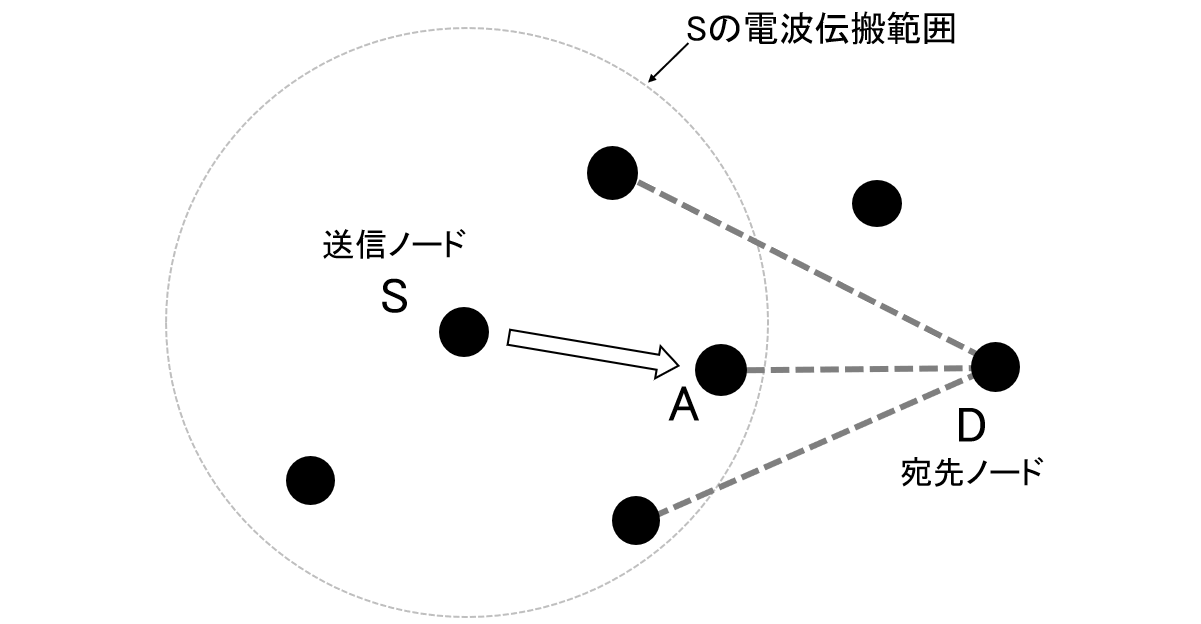
\includegraphics[scale=0.55]{figures/greedy.png}
  \caption{Greedy Forwarding\cite{shinato}}
  \label{fig:greedy}
\end{figure}

Greedy Forwardingでは局所最大問題と呼ばれる問題が生じてしまうことがある. 
\textbf{局所最大問題}とは, 図\ref{fig:local}に示すように, 送信ノードSの電波伝搬範囲内に
宛先ノードDが存在しない, かつ, 送信ノードSが自身の
電波伝搬範囲内で宛先ノードDに最も近い場合, 選択できる
ネクストホップが存在しなくなるという問題である.

\begin{figure}
  \centering
  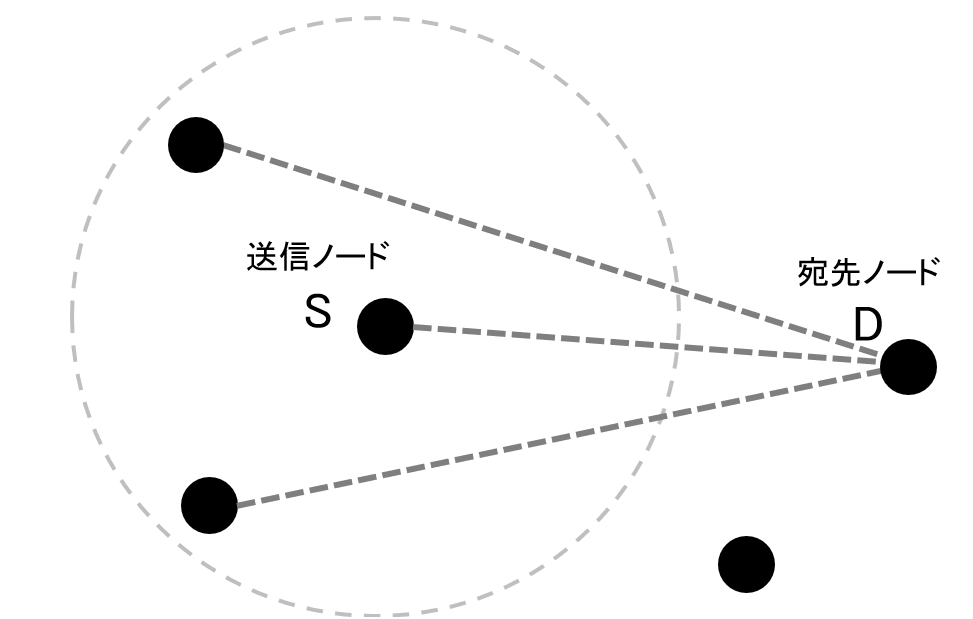
\includegraphics[scale=0.55]{figures/local.png}
  \caption{局所最大問題}
  \label{fig:local}
\end{figure}

\noindent {\Large\textbf{Perimeter Forwarding}}\\
Greedy Forwardingで局所最大問題が発生した場合に, 
Perimeter Forwardingが使用される. 
図1.5のように, 送信ノードSを中心に
\textbf{Right Hand Rule} に則って反時計回りにノードを探索し, 
最初に発見したノードをホップとして選択する方式である.

\textbf{図1.5を挿入}
\section{デジタル署名}
\textbf{デジタル署名}とは, 公開鍵暗号の仕組みを利用して作られた暗号技術であり, 
電子文書やメッセージの真正性と完全性を検証するために使用される. 
この技術は, データの信頼性を確保し, かつ, 送信者がデータの送信を否定できない
非否認性を提供する.\\
% \textbf{デジタル署名}とは, するための
% 暗号技術であり, 電子データの送信者を認証するとともに, 
% そのデータが通信途中で改ざんされていないことを保証する仕組みである. 
% この技術は, データの信頼性を確保し, 送信者がデータの送信を否定できない
% 非否認性を提供する.\\
\indent 一般に, デジタル署名は以下の3つのフェーズから構成される.

\begin{enumerate}
  \item \textbf{鍵生成}\\
  \indent 署名者(送信者)が署名に使用する鍵のペア, 
  すなわち検証鍵(公開鍵)と署名鍵(秘密鍵)を生成するフェーズである. 
  署名鍵は署名者が厳重に管理し, 秘密に保管する. 一方, 検証鍵は
  受信者や第三者に公開され, 署名の検証に用いられる.
  \item \textbf{署名生成}\\
  \indent メッセージ作成者(送信者)は, 署名対象のメッセージから
  ハッシュ関数を用いてハッシュ値を計算する. このハッシュ値は, 
  メッセージがわずかでも変更されると全く異なる値となるため, 
  メッセージが改ざんされていないこと(完全性)を検証するための
  重要な要素である. 続いて, メッセージ作成者は自身の署名鍵(秘密鍵)を
  使ってハッシュ値に署名を行う. 署名鍵がメッセージ作成者
  しか保持していないことと, メッセージ作成者以外が署名鍵を求めることは
  計算量的に困難なことから, 署名はメッセージの作成者が正当であること
  (真正性)を証明する役割を果たす. 
  \item \textbf{署名検証}\\
  \indent 検証者(受信者)は, 署名者が公開した検証鍵(公開鍵)を用いて
  署名を検証する. この検証プロセスにより, 署名が署名鍵と対になる
  検証鍵によって生成されたことを確認できるため, メッセージが正規の
  作成者によって署名され, 送信後に改ざんされていないことが保証される.
\end{enumerate}

デジタル署名にはさまざまなアルゴリズムが存在する. その中でも,    
\textbf{国立標準技術研究所(National Institute of Standards and Technology, NIST)}
による情報処理標準規格 FIPS に基づいて設計された
\textbf{ECDSA(Elliptic Curve Digital Signature Algorithm)}は, 
V2V通信のようなリアルタイム性やリソース制約が求められる環境に
適しているため, 先行研究\cite{shinato}で使用されていた. 
したがって, 本研究でも, ECDSA方式を用いて
シミュレーション実験をし, EdDSAと比較評価を行う. \\
以下に, ECDSAの概要を示す. \\[1em] 


% \noindent {\Large\textbf{DSA}}\\
% \textbf{DSA (Digital Signature Algorithm)}は, 1993 年に FIPS 186-4として
標準化された, DSS (Digital Signature Standard) の主要なアルゴリズムの
1つであった. なお, 2023 年の FIPS 186-5\cite{fips186-5} では,DSAは
新たにデジタル署名を行うことには推奨されないが, 標準策定以前に行われた
署名の検証には引き続き利用可能とされている.\\
\indent DSAの3つのフェーズにおける処理は以下の通りである.\\[0.5em]
\let\ltxlist\list
\begin{breakitembox}[l]{\textbf{鍵生成}}
   
  \begin{enumerate}[parsep=7pt]
    \item セキュリティパラメータとして整数 $L,N (L>N)$ を定める. 
    FIPS186-4では以下の4つの値の組が規定されている.
    \begin{center}
      $(L,N) = (1024,160), (2048,224), (2048,256), (3072,256)$
    \end{center}
    \item $N$ビットのランダムな素数$q(2^{N-1}<q<2^{N})$, 
    $L$ ビットのランダムな素数$p(2^{L-1}<q<2^{L})$ を選ぶ.
    ただし, $q$は$p-1$を割り切る素数とする.
    \item ランダムな整数$a<p-1$に対し,
    \[
      g\equiv a^{\frac{p-1}{q}}\pmod p
    \] 
    を計算する. ただし,$g=1$である場合は再度$a$を選び直す.
    \item ランダムな整数$x(1<x<q)$に対し,
    \[begin{equation}]
      y\equiv g^x\pmod p
    \]
    を計算する.
    \item $p,q,g$は専用のパラメータとして, $y$は検証鍵(公開鍵)として
    公開する. $x$は署名鍵(秘密鍵)として安全に管理する.
  \end{enumerate}
\end{breakitembox}
\vspace{1em}
\indent 任意長のメッセージ $M$ に対して, パラメータ$p, q, g$, 秘密鍵$x$, 
ハッシュ関数$H$ を用いて, 次のように署名を生成する.
\vspace{1em}
\let\ltxlist\list
\begin{breakitembox}[l]{\textbf{署名生成}}
   
  \begin{enumerate}[parsep=7pt]
    \item ランダムな整数 $k(1<k<q)$ を選ぶ.
    \item $r\equiv (g^k\pmod p)\pmod q$ を計算する. 
    ただし, $r=0$ の場合は再度 $k$ を選び直す.
    \item $s\equiv k^{-1}(H(M+xr))\pmod q$ を計算する.
    ただし, $s=0$ の場合は再度 $k$ を選び直す.
    \item $(r,s)$ をメッセージ$M$に対する署名とし, 
    $M$とともに受信者に送信する.
  \end{enumerate}
\end{breakitembox}
\vspace{1em}
メッセージ$M$に対する署名$(r, s)$を検証するには, パラメータ$(p,q,g)$, 
公開鍵$y$, ハッシュ関数$H$を用いて, 以下のアルゴリズムを実行する.
\vspace{1em}
\let\ltxlist\list
\begin{breakitembox}[l]{\textbf{署名検証}}
   
  \begin{enumerate}[parsep=7pt]
    \item 受け取った$(r,s)から, $$0<r<q$ かつ $0<s<q$ であることを確認する. 
    これを満たさない場合は署名を棄却する.
    \item $w\equiv s^{-1}\pmod q$ を計算する.
    \item $u_1\equiv wH(M)\pmod q$を計算する.
    \item $u_2\equiv rw\pmod q$ を計算する.
    \item $v\equiv (g^{u_1}y^{u_2}\pmod p)\pmod q$ を計算する.
    \item $v=r\pmod  q$ であれば, 署名を受理する. そうでなければ
    不正な署名とみなし, 棄却する.
  \end{enumerate}
\end{breakitembox}
\vspace{1em}
\indent 正当なメッセージと署名の組$(M, (r, s))$に対し, 
\[
  g^{u_1}y^{u_2}\equiv g^{u_1+xu_2} \equiv g^{H(M)+xr}w\equiv g^{k}\pmod p
\]
が成り立つ. これは 
\begin{align*}
  v &\equiv (g^{u_1}y^{u_2} \mod p) \mod q \\
    &\equiv (g^k \mod p) \mod q \\
    &\equiv r \mod q
\end{align*}
であることを示す.\\
\indent ここで, メッセージや署名に対し改ざんが行われたとしよう. 
攻撃者が, 署名検証条件 $v \equiv r \pmod{q}$ を
満たすように操作できた場合, その攻撃は成功したとみなされる. ただし, 
署名生成に使用される値には, 署名者しか知らない秘密の乱数$k$が
含まれており, この$k$は離散対数問題に基づいて計算されるため, 
十分なビット長を持つ$p$および$q$の下では, 改ざんを成功させることは
計算量的に極めて困難である.さらに, 署名生成プロセスではメッセージの
ハッシュ値$H(M)$が使用されており, このハッシュ値はハッシュ関数の
衝突困難性に依存している. したがって, 攻撃者が異なるメッセージ $M'$ を
生成し, そのハッシュ値が元のメッセージ $M$ と同じ $H(M') = H(M)$ と
なるようにすることも困難である. この性質により, 改ざんされたメッセージ
$M'$のハッシュ値は$H(M')\neq H(M)$となり, 
署名検証条件 $v \equiv r \pmod{q}$ が成立しなくなる.
また, 攻撃者がメッセージ$M$をそのままにして署名$(r, s)$を
改ざんした場合でも, 署名にはハッシュ値$H(M)$が埋め込まれているため, 
署名検証条件は満たされない. この結果, 署名検証アルゴリズムの最終段階で
署名が有効と判定される場合, 署名$(r, s)$もメッセージ$M$も
改ざんされていないことが保証される.



\noindent {\Large\textbf{ECDSA}}\\
\indent \textbf{ECDSA (Elliptic Digital Signature Algorithm)}は, 
DSA\cite{fips186-5}を楕円曲線暗号(Elliptic Curve Cryptography, ECC)を基盤として
改良したデジタル署名アルゴリズムである.
ECDSAは, 2000年に FIPS 186-2として標準化され, 
最新版であるFIPS 186-5\cite{fips186-5}でも採用されている.
ECDSAは, DSAよりも短い鍵長で同等の安全性を確保できるため, 
計算量が少なく, 低性能なデバイスでも高速な処理が可能であり, 
かつ演算規則の複雑さから攻撃者が鍵を推測することも困難である. \\
\indent この項では, ECDSAの理解に必要となる楕円曲線とその上での演算について
説明し, その後, ECDSAのアルゴリズムについて述べる.\\[1em]

\noindent{\large\textbf{楕円曲線}}\\
\indent 体$\mathbb{F}_p$($p$は素数)上で定義された楕円曲線とは以下の式で与えられる
代数曲線である.
\[
  y^2+a_1y+a_3y=x^3+a_2x^2+a_4x+a_6  (a_1,a_2,a_3,a_4,a_6\in\mathbb{F}_p)
\]
この式をWeierstrass方程式という\cite{安田}. 
特に, $p\neq 2,3$の場合, 以下の標準形に簡略化できることが知られている. 
\begin{equation}\label{weierstrass}
  y^2=x^3+ax+b  (a,b\in\mathbb{F}_p)
\end{equation}
\indent 楕円曲線(式(\ref{weierstrass}))の判別式$\Delta$が
\[
  \Delta=-16(4a^3+27b^2)\neq 0
\]
を満たすとき, 楕円曲線(式\ref{weierstrass})は\textbf{非特異}であるという. 
非特異である楕円曲線は, 尖点や自己交差点, 孤立点を持たないため, 
楕円曲線が非特異であることは, 後述する楕円曲線上の点に対する演算
(加算やスカラー倍)が矛盾なく定義されるために必要不可欠である.\\
\indent 楕円曲線上の点$P=(x,y)$のうち$x,y$がともに有限体
$\mathbb{F}_p$の元であるものを\textbf{有理点}という. また, 楕円曲線上には
\textbf{無限遠点}と呼ばれる特殊な点$\mathcal{O}$の存在を仮定し, これも楕円曲線上の
有理点の集合に含める. 有理点の集合は, 以下で述べる演算に関して
群の構造をもつ. 楕円曲線暗号方式では,この性質が利用される.\\[1em]
\noindent\textbf{楕円曲線上の点の加算}\\
\indent 楕円曲線上の点$P=(x_1,y_1)$と$Q=(x_2,y_2)$の加算 $P+Q$ を
以下のように定義する.
\begin{enumerate}
  \item[(i) ] 2点$P,Q$を通る直線が$y$軸と平行でない場合%(図1.6):
  \begin{enumerate}
    \item[1. ] 点$P,Q$を通る直線$L$を引く.
    \[
      L : y-y_1 = \frac{y_2-y_1}{x_2-x_1}(x-x_1)
    \]
    \item[2. ] $L$と楕円曲線$E$の交点を$R(x_3,y_3)$とする.
    \[
    \begin{aligned}
      x_3 &= \left(\frac{y_2-y_1}{x_2-x_1}\right)^2-x_1-x_2\\
      y_3 &= \frac{y_2-y_1}{x_2-x_1}(x_1-x_3)-y_1
    \end{aligned}
    \]
    \item[3. ] $R$の$x$軸対称な点$R'(x_3,-y_3)$が$P+Q$となる.
    \[
      P+Q=R'
    \]
  \end{enumerate}
  % {\LARGE\textbf{図1.6を挿入}}\\
  \item[(ii) ] 2点$P,Q$を通る直線$L$が$y$軸と平行である場合:\\
  \indent この場合, 直線$L$は2点$P,Q$以外で楕円曲線$E$と交わらない.\\ 
  \indent 無限遠点$\mathcal{O}$が$P+Q$となる.
  \[
    P+Q=\mathcal{O}
  \]
  \item[(iii) ] 2点$P,Q$が同一の点である場合%(図1.7):\\
  \begin{enumerate}
    \item[1. ] 点$P$における接線$L'$を引く. 
    \[
      L' : y-y_1 = \frac{3x_1^2 + a}{2y_1}(x - x_1)
    \] 
    \item[2. ] $L'$と楕円曲線$E$の交点を$R(x_3,y_3)$とする.
    \[
    \begin{aligned}
      x_3 &= \left(\frac{3x_1^2 + a}{2y_1}\right)^2-2x_1\\
      y_3 &= \frac{3x_1^2 + a}{2y_1}(x_1-x_3)-y_1
    \end{aligned}
    \]
    \item[3. ] $R$の$x$軸対称な点$R'(x_3,-y_3)$が$P+Q$となる.
    \[
      P+Q=2P=R'
    \]
  \end{enumerate}
  % {\Huge\textbf{図1.7を挿入}}
  \item[(iv) ] $P=\mathcal{O}$または$Q=\mathcal{O}$である場合:\\
  \indent 無限遠点は加算において加法単位元の役割を果たす.
  \[
  \begin{aligned}
    P+\mathcal{O}&=P\\
    \mathcal{O}+Q&=Q
  \end{aligned}
  \]    
\end{enumerate}
\vspace{0.5em}
\noindent\textbf{スカラー倍算}\\
\indent 正整数$k$による点$G$のスカラー倍$P=kG$は, 点$G$を$k$回加算した結果を表す.
\[
  P=kG=\underbrace{G+G+\cdots+G}_{k\text{回}}
\]
\indent ある基準点$G$に対し, $P = kG$となる楕円曲線上の点$P$が与えられたとき, 
$k$と$G$から$P$を求めるのは容易である. しかし, 逆に$G$と$P$から$k$を
求めるのは計算量的に困難であることが知られている. 
これを\textbf{楕円曲線上の離散対数問題(Elliptic Curve Discrete Logarithm Problem, ECDLP)}という.\\[1em]

\noindent{\large\textbf{ECDSAのアルゴリズム}}\\
\indent ECDSAの3つのフェーズにおける処理は以下の通りである.
\vspace{1em}
\let\ltxlist\list
\begin{breakitembox}[l]{\textbf{鍵生成}}
   
  \begin{enumerate}[parsep=7pt]
    \item 法となる素数$p$と, 楕円曲線$E$を選び, $E$上の基準点$G$を選ぶ.
    \item $d$を$2\leq d\leq n-1$の範囲からランダムに選び, 
    署名鍵(秘密鍵)として安全に管理する. ただし, $n$は$G$の位数である.
    \item $Q=dG$を計算し, $Q$を検証鍵(公開鍵)とする.
  \end{enumerate}
\end{breakitembox}
\vspace{1em}
\let\ltxlist\list
\begin{breakitembox}[l]{\textbf{署名生成}}
   
  \begin{enumerate}[parsep=7pt]
    \item $k$を$2\leq k\leq n-1$の範囲からランダムに選び, $kG$の
    $x$座標を$r$とする.
    \item メッセージ$M$に対し, ハッシュ関数$H$を用いて, $h=H(M)$を計算する.
    \item $s\equiv k^{-1}(h+dr)\pmod n$を計算する.
    \item $(r,s)$をメッセージ$M$に対する署名とし, 
    $M$とともに受信者に送信する.
  \end{enumerate}
\end{breakitembox}
\vspace{1em}
\let\ltxlist\list
\begin{breakitembox}[l]{\textbf{署名検証}}
   
  \begin{enumerate}[parsep=7pt]
    \item $(M,(r,s))$を受け取り, $h=H(M)$を計算する. 
    \item $u\equiv s^{-1}h\pmod n$, $v\equiv s^{-1}r\pmod n$を計算する.
    \item 楕円曲線上の点として, 
    \[
      Q'=(x',y')=uG+vQ
    \]
    を計算する.
    \item $Q'$の$x$座標$x'$が$r$と一致すれば, 署名を受理する.
    そうでなければ不正な署名とみなし, 棄却する.
  \end{enumerate}
\end{breakitembox}
\vspace{1em}
\indent 正当なメッセージと署名の組$(M, (r, s))$に対し, 
\begin{align*}
  Q'  &= uG + vQ\\
      &= s^{-1}hG + s^{-1}rQ \\
      &= s^{-1}hG + s^{-1}rdG \\
      &= s^{-1}hG + s^{-1}(sk-h)G \\
      &= s^{-1}(hG + skG - hG) \\
      &= s^{-1}skG \\
      &= kG
\end{align*}
が成り立つため, $Q'$の$x$座標が$r$と一致するかどうかを確認することで
署名検証が可能である.\\
\section{ns-3}
本研究では, シミュレーションツールとして\textbf{network simulator-3(ns-3)}
\cite{ns-3}を使用した. ns-3は, 離散事象ネットワークシミュレータであり, 
有線および無線通信プロトコルを含む多様なネットワークの
シミュレーションが可能なオープンソースソフトウェアである. 
ns-3のシステムは大きく分けて, シミュレーションの
実行を行う\textbf{ns-3 core}と, 実験の定義を行う
\textbf{simulation scenario}に分かれている. simulation scenarioには, 
特定の通信プロトコルやネットワーク技術 (Wi-FiやGPSRなど)を再現するための機能が
モジュール化されており, 複数のモジュールを組み合わることでシミュレーションを実現する. 
そのため, ユーザーは, 必要なモジュールを選択し, モジュール内で不足している部分を
適宜実装していくことで, 要件に応じたシミュレーションを実行することができる. 
開発言語はC++とPythonをサポートしている. \\
\indent ns-3では様々なコンテナと呼ばれるノードやネットワーク要素を効率的に
管理するためのデータ構造が存在し, それらを組み合わせて
プログラムを作成していく. 一般的には次の4つの主要なコンテナが使用される.
\begin{itemize}
  \item NodeContainer\\ 
  \indent ノードを管理するためのコンテナであり, 
  コンピュータやルータなど, 扱うデバイスが何であるかを示す. 
  \item DeviceContainer\\
  \indent 通信デバイスを管理するためのコンテナであり, 
  ノードがどのような通信機能をもつかを指定する. 
  \item InterfaceContainer\\
  \indent IPインターフェースを管理するためのコンテナであり, IPアドレスや
  サブネットマスクなどの情報を保持する.
  \item ApplicationContainer\\
  \indent アプリケーションレイヤのプログラムやサービスを管理するための
  コンテナであり, HTTPサーバやUDPアプリケーションなどが用意されている.
\end{itemize}

